\documentclass[
  bibliography=totoc,     % Literatur im Inhaltsverzeichnis
  captions=tableheading,  % Tabellenüberschriften
  titlepage=firstiscover, % Titelseite ist Deckblatt
]{scrartcl}

% Paket float verbessern
\usepackage{scrhack}

% Warnung, falls nochmal kompiliert werden muss
\usepackage[aux]{rerunfilecheck}

% unverzichtbare Mathe-Befehle
\usepackage{amsmath}
% viele Mathe-Symbole
\usepackage{amssymb}
% Erweiterungen für amsmath
\usepackage{mathtools}

% Fonteinstellungen
\usepackage{fontspec}
% Latin Modern Fonts werden automatisch geladen
% Alternativ zum Beispiel:
%\setromanfont{Libertinus Serif}
%\setsansfont{Libertinus Sans}
%\setmonofont{Libertinus Mono}

% Wenn man andere Schriftarten gesetzt hat,
% sollte man das Seiten-Layout neu berechnen lassen
\recalctypearea{}

% deutsche Spracheinstellungen
\usepackage[ngerman]{babel}


\usepackage[
  math-style=ISO,    % ┐
  bold-style=ISO,    % │
  sans-style=italic, % │ ISO-Standard folgen
  nabla=upright,     % │
  partial=upright,   % │
  mathrm=sym,        % ┘
  warnings-off={           % ┐
    mathtools-colon,       % │ unnötige Warnungen ausschalten
    mathtools-overbracket, % │
  },                       % ┘
]{unicode-math}

% traditionelle Fonts für Mathematik
\setmathfont{Latin Modern Math}
% Alternativ zum Beispiel:
%\setmathfont{Libertinus Math}

\setmathfont{XITS Math}[range={scr, bfscr}]
\setmathfont{XITS Math}[range={cal, bfcal}, StylisticSet=1]

% Zahlen und Einheiten
\usepackage[
  locale=DE,                   % deutsche Einstellungen
  separate-uncertainty=true,   % immer Unsicherheit mit \pm
  per-mode=symbol-or-fraction, % / in inline math, fraction in display math
]{siunitx}

% chemische Formeln
\usepackage[
  version=4,
  math-greek=default, % ┐ mit unicode-math zusammenarbeiten
  text-greek=default, % ┘
]{mhchem}

% richtige Anführungszeichen
\usepackage[autostyle]{csquotes}

% schöne Brüche im Text
\usepackage{xfrac}

% Standardplatzierung für Floats einstellen
\usepackage{float}
\floatplacement{figure}{htbp}
\floatplacement{table}{htbp}

% Floats innerhalb einer Section halten
\usepackage[
  section, % Floats innerhalb der Section halten
  below,   % unterhalb der Section aber auf der selben Seite ist ok
]{placeins}

% Seite drehen für breite Tabellen: landscape Umgebung
\usepackage{pdflscape}

% Captions schöner machen.
\usepackage[
  labelfont=bf,        % Tabelle x: Abbildung y: ist jetzt fett
  font=small,          % Schrift etwas kleiner als Dokument
  width=0.9\textwidth, % maximale Breite einer Caption schmaler
]{caption}
% subfigure, subtable, subref
\usepackage{subcaption}

% Grafiken können eingebunden werden
\usepackage{graphicx}

% schöne Tabellen
\usepackage{tabularray}
\UseTblrLibrary{booktabs, siunitx}

% Verbesserungen am Schriftbild
\usepackage{microtype}

% Literaturverzeichnis
\usepackage[
  backend=biber,
]{biblatex}
% Quellendatenbank
\addbibresource{lit.bib}
\addbibresource{programme.bib}

% Hyperlinks im Dokument
\usepackage[
  german,
  unicode,        % Unicode in PDF-Attributen erlauben
  pdfusetitle,    % Titel, Autoren und Datum als PDF-Attribute
  pdfcreator={},  % ┐ PDF-Attribute säubern
  pdfproducer={}, % ┘
]{hyperref}
% erweiterte Bookmarks im PDF
\usepackage{bookmark}

% Trennung von Wörtern mit Strichen
\usepackage[shortcuts]{extdash}

\author{%
  Vincent Wirsdörfer\\%
  \href{mailto:vincent.wirsdoerfer@udo.edu}{authorA@udo.edu}%
  \and%
  Joris Daus\\%
  \href{mailto:joris.daus@udo.edu}{authorB@udo.edu}%
}
\publishers{TU Dortmund – Fakultät Physik}


\begin{document}
\section{Versuchsaufbau}
\label{sec:Versuchsaufbau}

Das Kernelement des Versuches ist ein Glaszylinder mit aufgedruckter Längenskala. In diesem Glaszylinder befindet 
sich eine radioaktive Strahlungsquelle und ein Halbleiter-Detektor. Die Strahlungsquelle ist auf einem verschiebbaren Halter 
positioniert, sodass der Abstand zwischen Präparat und Detektor variiert werden kann. Bei dem hier betrachteten Detektor 
handelt es sich um einen Halbleiter-Sperrschichtzähler, welcher ähnlich zu einer Diode funktioniert. Dieser besteht im 
Wesentlichen aus einer p- und n-dotierten Schicht, welche durch eine \enquote{Verunreinigung} des Halbleitermaterials 
hervorgerufen wird. Werden beispielsweise Bohr- und Phosphor-Atome in einen Silizium-Halbleiter eingesetzt, so entshen aufgrund 
der jeweiligen Elektronenkonfiguration der Fremdatome Bohr und Phosphor zusätzliche \enquote{Elektronen-Loch-Paare} (p-Dotierung)
und Elektronen (n-Dotierung). Zwischen diesen Schichten befindet sich eine ladungsfreie Zone, die sogenannte 
\emph{Verarmungszone}. Ähnlich einer Diode gibt es hierbei eine Sperrrichtung und eine Durchlassrichtung für sich bewegende Elektronen.
Wird nun eine Spannung im Sinne der Sperrrichtung angelegt, entsteht ein zusätzliches elektrisches Feld, welches die Verarmungszone 
vergrößert. Fallen nun die ionisierten Teilchen der $\alpha$-Strahlungsquelle in die eben genannte Zone ein, werden weitere
Elektronen-Loch-Paare erzeugt, welche in Folge des elektrischen Feldes einen Stromimpuls bedingen. Dieser Impuls wird nun von 
einem Vorverstärker verstärkt und an einen Vielkanalanalysator weitergeleitet. Hier werden die detektierten Impule in Form eines Histogramms visualisiert. 
Die genaue Verknüpfung der Geräte wird in der unten stehenden Abbildung \ref{fig:Aufbau} dargestellt. Wie in Kapitel \ref{sec:Theorie} bereits erläutert,
wird zur Bestimmung der Reichweite der Teilchen die Proportionalität zum herrschenden Druck angewendet. Zur Regulierung des Drucks dient eine Vakuumpumpe 
und zwei Ventile. Der Betrag des Drucks lässt sich am Druckmessgerät navigieren und ablesen.

\begin{figure}[H]
    \centering
    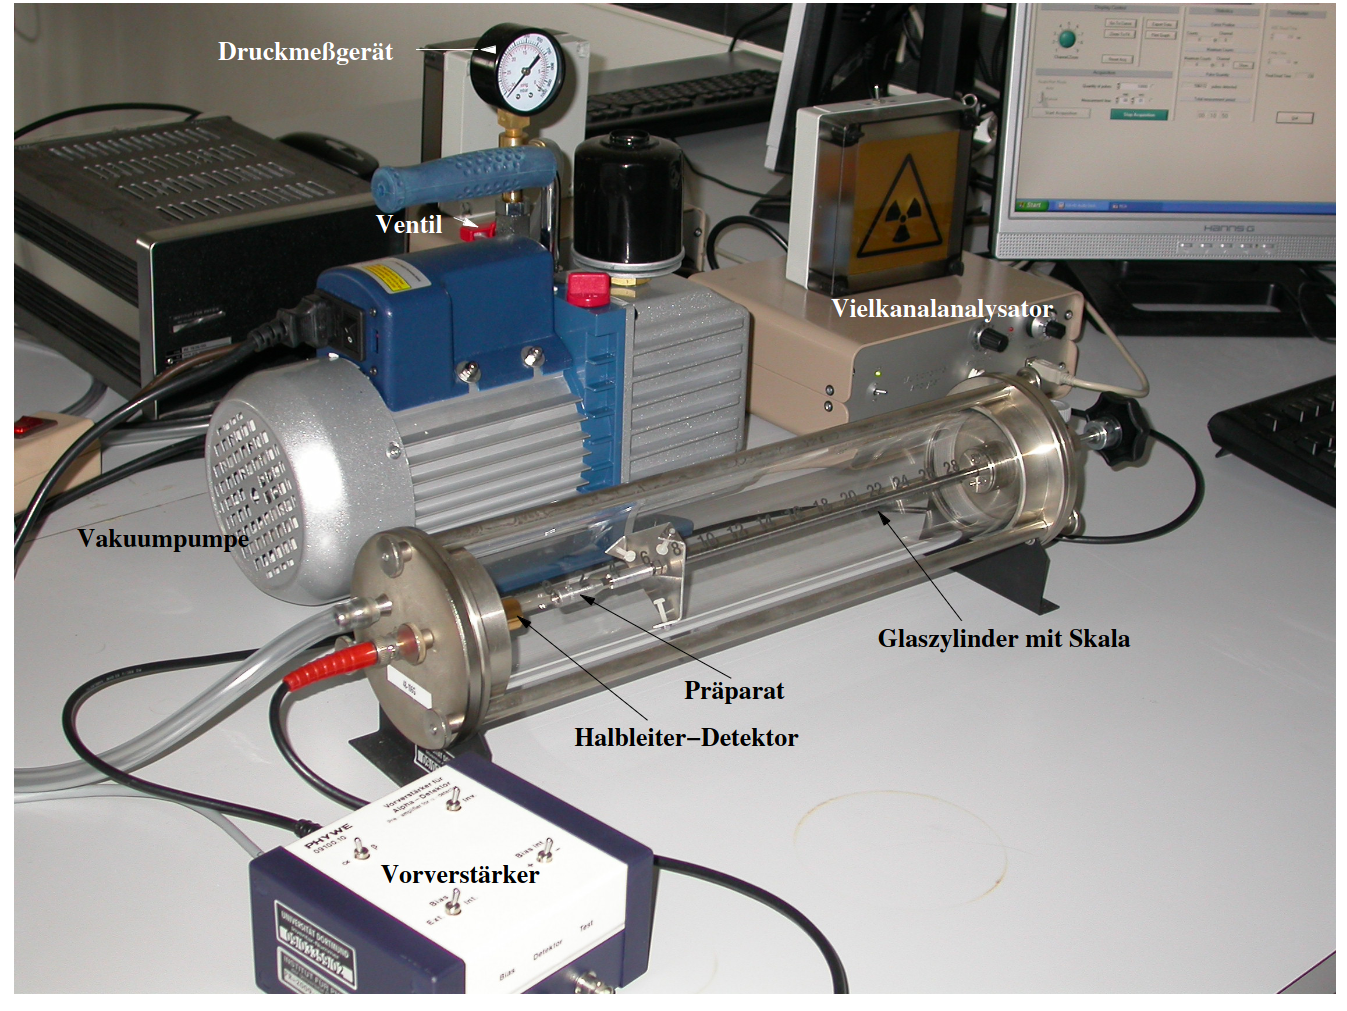
\includegraphics[height=7cm]{Aufbau.png}
    \caption{Apparaturdarstellung des Versuchs\cite{Versuchsanleitung_v701}.}
    \label{fig:Aufbau}
\end{figure}

\section{Versuchsdurchführung}
\label{sec:Versuchsdurchführung}

Zu Beginn des Versuchs wird die korrekte Verkabelung der Gerätschaften überprüft. Im Anschluss wird ein Absatnd von \qty{4}{\centi\meter} zwischen 
Strahlungsquelle und Detektor anhand der Längenskala eingestellt. Zusätzlich wird die Vakuumpumpe aktiviert und das Belüftungsventil geschlossen, 
sodass ein Vakuum kreiert werden kann. Sobald ein Druck von $p = \qty{0}{\milli\bar}$ erreicht ist, wird das Ventil von der Pumpe zum Zylinder 
geschlossen und die Pumpe erneut deaktiviert. Nun kann das Computerprogramm \emph{MCA} gestartet und eingestellt werden. Die Messzeit beträgt in 
Versuchsreihe 2 Minuten. Durch betätigen eines Buttons wird eine Messung gestartet, in welcher die detektieren Impulse analysiert werden. Nachdem 
die Messzeit von 2 Minuten überschritten ist, können die detektierten Impulse, sowie der \emph{Channel} mit den meisten Impulsen notiert. Daraufhin 
wird der Druck um \qty{50}{\milli\bar} erhöht, indem das Belüftungsventil leicht geöffnet wird. Bei Erreichen des gewünschten Drucks wird das Ventil
geschlossen und die Messung wieder gestartet. Diese Prozedur wird so lange wiederholt, bis der Peak des Histogramms durch die Bereinigungsfilter 
eingeschränkt wird.\\

\noindent Im Anschluss wird exakt diese Messung für einen veränderten Abstand $x_0 = \qty{5}{\centi\meter}$ zwischen Detektor und Präparat durchgeführt.
Außerdem soll die Statistik des radioaktiven Zerfalls untersucht werden. Hierzu wird im Programm eine Messzeit von \qty{10}{\second} eingestellt 
und die zum vorherigen Aufgabenteil identische Messung 100-mal ausgeführt. Ist diese Messreihe ebenfalls abgeschlossen, können die Geräte abgeschaltet
und der Computer heruntergefahren werden.   

\section{Messwerte}
\label{sec:Messwerte}



\end{document}

